
\documentclass[a4paper,10pt]{article}
\usepackage{multicol}
 \usepackage[pdftex]{graphicx}
\usepackage{algorithmic}
\usepackage{a4wide}

\newenvironment{figurehere}
{\def\@captype{figure}}
{}
\makeatother


\begin{document}
%
% paper title
% can use linebreaks \\ within to get better formatting as desired
\title{Dynamical Handling of Straddle Carriers Activities on a Container Terminal in Uncertain Environment \\ \textit{- A Swarm Intelligence approach -}}
%
%
% author names and IEEE memberships
% note positions of commas and nonbreaking spaces ( ~ ) LaTeX will not break
% a structure at a ~ so this keeps an author's name from being broken across
% two lines.
% use \thanks{} to gain access to the first footnote area
% a separate \thanks must be used for each paragraph as LaTeX2e's \thanks
% was not built to handle multiple paragraphs
%

\author{Stefan~Balev, Fr\'{e}d\'{e}ric~Guinand, Ga\"{e}tan~Lesauvage, Damien~Olivier
}

% note the % following the last \IEEEmembership and also \thanks -
% these prevent an unwanted space from occurring between the last author name
% and the end of the author line. i.e., if you had this:
%
% \author{....lastname \thanks{...} \thanks{...} }
%                     ^------------^------------^----Do not want these spaces!
%
% a space would be appended to the last name and could cause every name on that
% line to be shifted left slightly. This is one of those "LaTeX things". For
% instance, "\textbf{A} \textbf{B}" will typeset as "A B" not "AB". To get
% "AB" then you have to do: "\textbf{A}\textbf{B}"
% \thanks is no different in this regard, so shield the last } of each \thanks
% that ends a line with a % and do not let a space in before the next \thanks.
% Spaces after \IEEEmembership other than the last one are OK (and needed) as
% you are supposed to have spaces between the names. For what it is worth,
% this is a minor point as most people would not even notice if the said evil
% space somehow managed to creep in.



% The paper headers
%\markboth{Journal of \LaTeX\ Class Files,~Vol.~6, No.~1, January~2007}%
%{Shell \MakeLowercase{\textit{et al.}}: Bare Demo of IEEEtran.cls for Journals}
% The only time the second header will appear is for the odd numbered pages
% after the title page when using the twoside option.
%
% *** Note that you probably will NOT want to include the author's ***
% *** name in the headers of peer review papers.                   ***
% You can use \ifCLASSOPTIONpeerreview for conditional compilation here if
% you desire.




% If you want to put a publisher's ID mark on the page you can do it like
% this:
%\IEEEpubid{0000--0000/00\$00.00~\copyright~2007 IEEE}
% Remember, if you use this you must call \IEEEpubidadjcol in the second
% column for its text to clear the IEEEpubid mark.



% use for special paper notices
%\IEEEspecialpapernotice{(Invited Paper)}




% make the title area
\maketitle


\begin{abstract}
%\boldmath
    The CALAS project consists in a laser measure system allowing to localize precisely straddle carriers location in a box terminal. The information given by such a tool makes an optimization possible. In fact, a box terminal is an open system subject to dynamism, so many events can occur. They concern containers arrivals and departures. Within the terminal, straddle carriers are trucks which are able to carry one container at a time in order to move it through the terminal. We aim to optimize the straddle carriers handling to improve the terminal management. Moreover, missions come into the system in an unpredictable way and straddle carriers are handled by human. They can choose to follow the schedule or not. For these reasons, the exact state of the system, i.e the exact location of boxes is unknown. The optimizing system that we try to build must be fail-safe and adaptive. So, in this context, how to devote a mission to a straddle carrier ? We propose a simulation approach using a meta-heuristic based on Ant Colony to resolve the scheduling problem.
\\
\end{abstract}
% IEEEtran.cls defaults to using nonbold math in the Abstract.
% This preserves the distinction between vectors and scalars. However,
% if the journal you are submitting to favors bold math in the abstract,
% then you can use LaTeX's standard command \boldmath at the very start
% of the abstract to achieve this. Many IEEE journals frown on math
% in the abstract anyway.

% Note that keywords are not normally used for peerreview papers.
%\begin{keywords}
 swarm intelligence, colored ant colony system, dynamic graph, multiple criteria optimization.
%\end{keywords}
\begin{multicols}{2}
\section{System description}

The CALAS project aims at localizing precisely handling trucks on a box terminal. It uses a laser measure system and a software which allows to deal with the data sent by lasers. This project is the result of a collaboration between \textit{Laser Data Technology Terminal} company and the \textit{Terminaux de Normandie} company. The goal of the CALAS project is to know the state of the terminal in real time, meaning both containers and trucks location.
	
A box terminal is divided into three main areas. Each part is a set of boxes rows where containers can be stacked up and these areas are linked by oriented roads. The first area is beside a channel where ships can tie to the dockside. It is an area bound to prepare the ship load or unload. The second area is used to load or unload trucks. The third part is a storing area linking the two others. Containers are moved into this area when a ship or a truck is unloaded, and containers are moved from this area when a ship or a truck is loaded. So, there are three kinds of missions:

\begin{itemize}
	\item Preparing a ship loading / unloading
	\item Preparing a truck loading / unloading
	\item Optimizing storing area
\end{itemize}
		
The box terminal is an open system subject to dynamism. In fact, though a set of missions is known before starting the schedule, the main parts come into the system when the schedule has already been established. Moreover, trucks arriving time is not precisely known enough to forecast container delivery. If the truck is late, straddle carriers must wait for it to complete the mission, meanwhile, it can not accomplish another mission. Human behavior also affects the system because straddle carriers are handled by human drivers who can choose to follow the schedule or not.

\section{Vehicle Routing Problems classes}
 
Vehicle routing problems (VRP) are very common in some industrial processes, therefore, they are deeply studied. One or many vehicles must start from the depot, visit a list of customers, delivering (or picking-up) some goods, and coming back to the depot. The aim is to minimize the vehicle's routes. Many different subproblems belongs to the VRP class, such as capacitated Vehicle Routing Problem (CVRP) or Vehicle Routing Problem with Pickup and Delivery (VRPPD) by instance. Every subproblem contains a little variation of the main one, for example, it can have many depots, or vehicles must respect time windows... We distinguish static instances of these problems from the dynamics ones because the way to solve them are different.

\subsection{Vehicle Routing Problem (VRP)}
The Vehicle Routing Problem with Time Windows (see \cite{Bianchi00}) (VRPTW) consists in visiting a set of cities by a set of capacitated vehicles, optimizing path length. For instance, an Italian factory produces toys. It has to deliver a set of stores in order to make the goods sold. These stores are spread all over the country and goods are carried by trucks. Trucks capacity is restricted and they all start from the factory depot. Deliveries can only be done during a defined time interval. If a truck comes too early, it will have to wait. A solution to this problem should minimize the global length of the trucks runs.\\

The Dynamic VRPTW (DVRPTW) includes dynamism of the new orders. For the Italian factory example, if the stores can ask for deliveries when an already scheduled plan is running, then this problem belongs to DVRPTW class.

\subsection{Pickup and Delivery Problem (PDP)}
According to Berbeglia in \cite{Berbeglia07}, PDP contains 3 subclasses :\\

\subsubsection{Many to Many Pickup and Delivery Problems (M-MPDP) }

Here, the vehicles routes trend to pickup many objects to many locations. This kind of problem still relatively neglected because it is not frequently present in real situation.\\ %I can develop here if I need to fill the blanks...

\subsubsection{One to Many to One Pickup and Delivery Problems (1-M-1PDP) }

In this class, there are 2 different directions for the goods. They are first delivered to the customer. When the customer have done with them, he will ask for bringing back the goods to the depot. These problems must be with single or combined demands. In the first case, each customer ask for a delivery OR a pickup. With combined demands, a same customer can ask for both a delivery and a pickup.\\

\subsubsection{One to One Pickup and Delivery Problems (1-1PDP) }

This is the main subclass of Pickup and Delivery Problem, meaning the most frequently encountered problem in real life. It deals with picking-up one object at one location and delivering it to one destination. The main problem of this class is the Vehicle Routing Problem with Pickup and Delivery (VRPPD). In this problem, we have to compute the best routes for a fleet of vehicles in order to move objects on the graph. Every routes has to start and to end at the depot. It is not a 1-M-1PDP because here, each object $o$ has its own pickup and delivery location.\\%!!!! Explain it better !!!

When the problem deals with people, it is called Dial-A-Ride Problem (DARP). Some particular cases of VRPPD problems like the Stacker Crane Problem (SCP) are also common in practical life. This is a single vehicle with unit capacity problem. In an other subproblem, vehicles are allowed to temporarily drop their loads on specials locations called transshipment points to be able to better answer customers demands faster. This is called Vehicle Routing Problem with Pickup and Delivery and Transshipment.\\

When some request are not known in advance these static problems below may become dynamic. Those Dynamic Pickup and Delivery Problems (see \cite{Mitrovic01,Mitrovic04,Mitrovic98}) (DPDP or DVRPPD) consist in optimizing vehicles routes in order to pickup a load somewhere, then to deliver it to its destination, adapting these routes to the new incoming orders without recomputing from scratch. Most of the time, DVRPPD has to handle time windows (DVRPPDTW). Indeed, to start a mission, vehicles have to wait the beginning of its time window. If it is not respected, the vehicle will have to wait for the right time and, meanwhile this vehicle becomes useless.\\

\subsection{A new problem}

Our problem belongs to the Dynamic Vehicle Routing Problem with Pickup and Delivery and Time Windows (DVRPPD-TW). Several vehicles (straddle carriers) of unit capacity must accomplish missions (by moving containers within the box terminal). They also can use transshipment location to make the tasks more efficient. Straddle carriers can start from anywhere, ie. they don't have to start from the depot. If a vehicle comes too early for picking up or delivering a container, it will have to wait the beginning of the missions time window. Furthermore, if a straddle carrier is late, meaning its time window is now closed, the mission must be aborted and a new one dealing with the same box will appears into the system.\\

Three interconnected problems must be solved:
\begin{itemize}
	\item Minimize straddle carriers moves : shortest path problem
	\item Minimize ressources : clustering problem
	\item Minimize customers delays : scheduling problem
\end{itemize}

In order to realize a good scheduling, the system must integrate the shortest path concept. In the same way, scheduling shortest paths trends to reduce straddle carriers moves. Moreover, we have to define a quality of service level to satisfy customers while lowering operation costs. This is a dynamic large scale problem which requires a real time solution. We tried to develop an online algorithm based on Ant Colony Optimization (see \cite{Dorigo91,Dorigo97}) and more precisely on a colored version of this swarm algorithm (see \cite{Bertelle02}).

\section{Ant Colony and Straddle Carrier Handling}
Ant Colony (see \cite{Dorigo91,Dorigo97}) is a meta-heuristic which makes a solution appear thanks to the run of artificial ants into the solution space. The system is self-regulated. In fact, ants spread pheromone according to the solution quality (positive feedback) but the pheromone tracks evaporate progressively (negative feedback). The positive feedback makes the algorithm converge to a quality solution, and the negative feedback prevent it to block into a local extreme.

Ant Colony with one colony provides a sorted list of missions to accomplish (see \cite{Montemanni04,Bullnheimer97,Bullnheimer99}). The problem is to set a mission to a specific straddle carrier.

We have proposed to employ a solution using colored ants (see \cite{Bertelle02}). In our model, every straddle carrier represent a colony with its own color. Convergence is assured by the fact that ants are attracted by the pheromone of their own colony and repulsed by the pheromones of foreign colonies. These mechanisms will provide a sorted list of missions per every straddle carrier.

\subsection{Modelling}

The problem can be conceptualized as such:
\begin{itemize}
	\item let $M$ the set of missions to schedule. Every mission has a defined time window. We say that mission $m_i$ is prior to mission $m_j$ if the time window of $m_i$ starts before the one of $m_j$
	\item let $G$($V,A$) an oriented graph where $V$ is the set of vertices and $A$ the set of arcs.
	\item $\forall \; m \in M$, $\exists$ $v \in V$
	\item $\forall$~$c_i$~$\in$~$C$, where $C$ is the set of straddle carriers, $\exists$~$v_{k_i}$~$in$~$V$. $\forall$~$v$~$\in$~$V$, $\exists$~$a(v_{k_i},v)$~$\in$~$A$.
	\item $\exists$ $a_{c_i}(v_i , v_j) \in A$, if $m_i$ is prior to $m_j$ and if $m_i$ and $m_j$ can be executed by the vehicle $c_i$.	
	\item $\forall$ $v$, $\exists$~$e(h_i , v_j)$~$\in$ $E$, if $m_i$ is prior to $m_j$	
\end{itemize}

\begin{figurehere}
	\begin{center}
	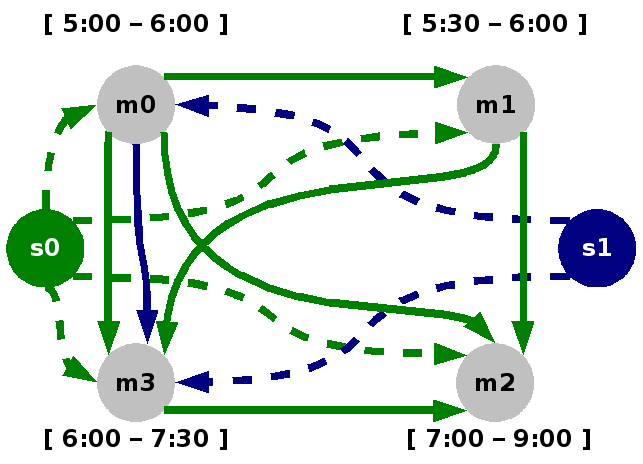
\includegraphics[width=\textwidth]{Shemas/missionGraphComplet.png}
	%\caption{Mission graph for 2 straddle carriers and 4 missions}
	\label{missiongraph}	
	\end{center}	
\end{figurehere}

In this way, a graph is set and ants colony system can be run to make the solution appears (see Fig. \ref{missiongraph}). The main algorithm is described on Fig. \ref{algo}. \\

\begin{figurehere}
\fbox{\begin{minipage}{0.45\textwidth}
	\begin{algorithmic}[1]
		\FORALL{colony c}
			\FORALL{ant of colony c}
				\STATE choose an unvisited destination according to the pheromone track
				\STATE move towards it according to the ant speed
				\STATE spread pheromone according to the destination quality
			\ENDFOR
		\ENDFOR
		\STATE evaporation
	\end{algorithmic}	
	
\end{minipage}}
%	\caption{Colored Ant System main algorithm}
	\label{algo}
\end{figurehere}


\subsection{Assets and weaknesses of Ant Colony}
Regarding the size of the solution space and the real time constraint, a metaheuristic is relevant for solving this problem. \\

The main asset of ant colony is to provide an anytime solution. It is an online algorithm which always tends to fit the problem whatever happens. %Whatever IT happens ?%
Indeed, on one hand, ants reinforce the pheromone rates to get closer to the best solution. On the other hand, at the same time, evaporation process provides a feed back control of the algorithm by preventing it to get stuck into a local optimum and allowing dynamic events to be handled.\\

Ant colony deals with evaporation, solution evaluation, ants quantity and speed, dynamic events, etc... It makes a lot of parameters. Here is a major weakness of this metaheuristic. Solution quality closely depends on these interdependent settings. %Tell how difficult it is to optimize these damn parameters before running several runs !
Although optimizing those parameters is a whole subject of research, we have been trying to make them self-adaptive. We use a local based method to adapt some of these parameters online.

\subsection{Division of labour}
As there are several distinct colonies in a local and distributed system, there is no way to use a pheromone spreading process based on a global characteristic. In fact, in this architecture, a colony can not evaluate the quality of its own solution compared with the ones of the other colonies. So, we must use the same pheromone spreading process for each colony. However, we are able to adapt the quantity of pheromone spread by ants of a colony according to the corresponding vehicle skill for a task. Indeed, in a fleet of $n$ vehicles, we can increase the quantity of pheromone spread by a vehicle $v_i$ ($i \in [1..n]$) for tasks concerning a specific area in the box terminal and decrease the quantity spread for the tasks located into the others area. At the same time, we do the opposite for a vehicle $v_j$  ($\forall j \neq i$). In this way, we try to specialize the vehicle in a kind of tasks and we are able to regulate these quantities by taking into account both the preference and the distance criteria.\\

This regulation keeps the benefit of allowing this specialized vehicle to take a mission for which it is not specialized. It is really important in some cases where the number of missions is high because this regulation prevents the system from having unused vehicles in an area of the terminal and unaffected missions, close of the end of their time window, in an other area. In this way, we are getting close to reproduce the division of labour in castes of a real ant colony.

\subsection{Reducing resources}
%How does it works
Always in a cost lowering purpose, we try to decrease the number of straddle carriers in the system. Our current solution to the entire problem tends to distribute the missions upon all the vehicles. So, every vehicle has almost the same activity rate. But if this rate is under a defined target, it is possible to conclude that a vehicle could be removed. Otherwise, if the rate is greater than the target, it is possible to say that a new vehicle should be added to the fleet.\\

%How to compute the target rate
The target rate must be computed by taking into account several facts. First, it has to deal with the quality of service. Indeed, the system must answer the request before the end of their time windows. Furthermore, if a vehicle is ready to serve several missions before the beginning of their time windows, it means that this vehicle is maybe superfluous, and so that the target rate must be raised. On the other hand, the target rate has to deal with other criteria like the covered distance of a vehicle per mission or the ratio between the number of vehicles and the number of missions, and it has to set these criteria against the penalties of transcended time windows. Measuring the time of inactivity of every straddle carrier may also lead the optimization. Concerning this last criterion, we must interrelate the time of inactivity with the penalties of transcended time windows.\\

%And what about dynamicity on ressources
So as for the missions arrivals into the system, the number of vehicles is subject to dynamicity. A vehicle can break down and then must be sent to the maintenance. In function of the failure seriousness, we can estimate the time needed to repair the vehicle and so make it available for routing. We take a rate of fault into account for optimizing the number of vehicles into the system because if this number is as low as possible without transcending some time windows, it will become too low if one vehicle of the fleet break down.

\section{Simulator}
%Introduction : 2 parts
The simulator has two main parts. The first one is the terminal simulation (see Fig. \ref{tview}), and the second one is the Colored ant Colony Optimization System (see Fig. \ref{acoview}).
%% 1st part
The first part contains an implementation of the terminal structure and components. Roads and crossroads provide the network of the terminal on which straddle carriers will be able to go. Some of these roads may contain containers. Quay crane locations are represented by these specials roads, so as the trucks handling locations. This terminal is built at the very beginning of the simulation. A scenario file is read to set the terminal configuration.
%% 2nd part
The second part of the simulator contains the algorithmic view of the simulation, i.e the dynamic mission graph. In this way, it shows how the missions are chosen by the vehicles. This part of the simulator uses GraphStream\footnote{http://graphstream-project.org/} toolkit which allows to handle dynamic graph easily (see \cite{Dutot2007}).\\

% Discrete motor and dynamicity
The simulator uses a discrete motor which has to iterate every object of the simulation on every single step. Throughout the simulation, the scenario file is read and some dynamic events are sent back to both terminal and Ant Colony views. In this way, the system can simulate the dynamicity %??? Can I say so ?
of the incoming missions and of the vehicles availability.\\

%% Measure of dynamicity
In order to have relevant tests and results, we have to define several levels of dynamicity. But how to value a such level? In \cite{larsen00}, Allan Larsen point out two main ways to measure the degree of dynamicity.\\

%%%dod
First, the degree of dynamism ($dod$) (see \cite{Lund96}) is the ratio between the number of dynamical requests and the overall ones. The main weakness of this measure is that it does not take  into account the arrival time of these requests into the system. Indeed, with $dod$ if the requests come into the system at the beginning of the day, the system is as dynamic as if they come late in the day. Yet, the later these requests are known, the shorter is the delivery delay. This lateness impacts on the performance of the system.\\

%%%edod
For this reason, Larsen and al. in \cite{larsen00} defined the effective degree of dynamism ($edod$) by this formula : \\
\begin{equation}
	edod\;=\; \frac{\sum_{i=1}^{\eta_d}\frac{t_i}{T}}{\eta_d+\eta_s}
	%\label{edod}
\end{equation}
Here, $\eta_s$ and $\eta_d$ are respectively the number of static and dynamic requests, and $t_i$ is the time $i$ (with $0 < t_i < T $) and $T$ is the time of the simulation end. These measure take into account the average of the incoming time of the requests into the system. The more the dynamical requests come late, the more $edod$ will be high. If $edod=0$, then the system is totally static. Else, if $edod = 1$, then the system is purely dynamic.


% Mission schedulling
Every straddle carriers on the terminal simulation received a schedule from the Colored Ant Colony System. Then they act in function of it and move to their pick-up location. Once they have picked-up their container, they move to the delivery location to achieve their mission. At the same time, the mission graph is dynamically updated and the colored ants keep colonizing it.\\

\begin{figurehere}
\fbox{\begin{minipage}{0.45\textwidth}
	\begin{center}
		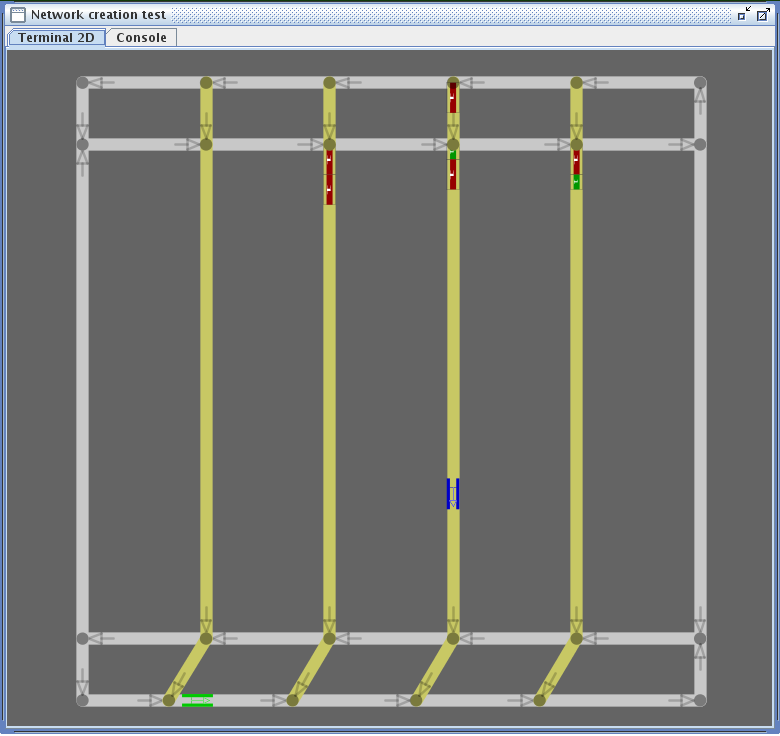
\includegraphics[width=\textwidth]{Shemas/terminal.png}
	\end{center}
\end{minipage}}
%\caption{Terminal view in the simulator}
\label{tview}
\end{figurehere}

Simulator gives information about each mission like its length, container, straddle carrier 

\begin{figurehere}
\fbox{\begin{minipage}{0.45\textwidth}
 	\begin{center}
		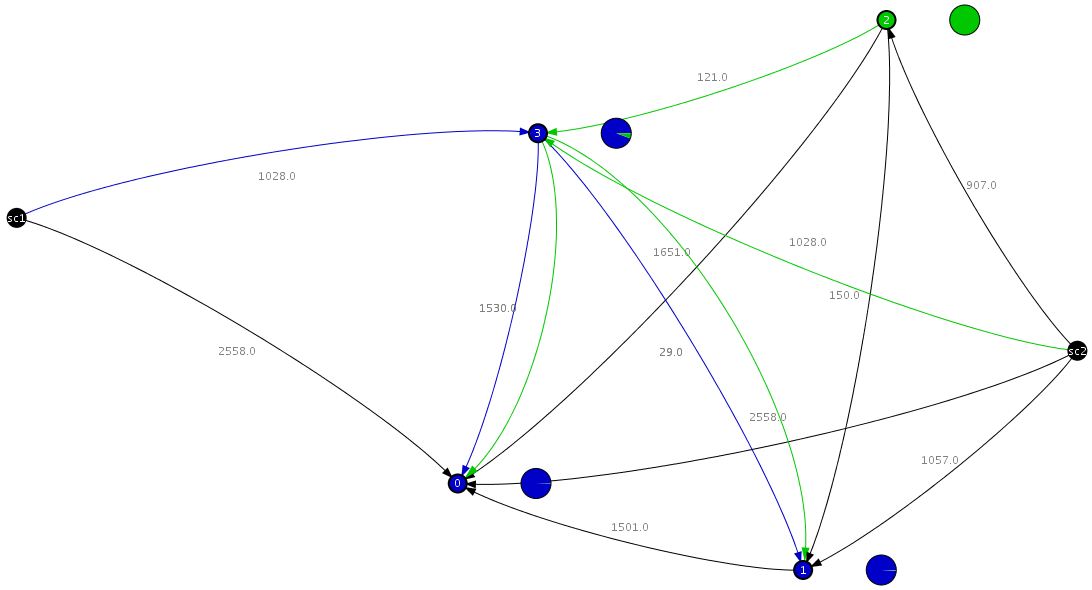
\includegraphics[width=\textwidth]{Shemas/aco.PNG}
	\end{center}
\end{minipage}}
%	\caption{Mission graph view in the simulator}
	\label{acoview}
\end{figurehere}

% 	\section*{Results}
% 	Coming soon !

\section{Conclusion}

The problem to solve belongs to the Dynamic Pickup and Delivery Problem with Time Windows class. However, it does not exactly fit. So it is an original unsolved problem. We propose to solve it using swarm intelligence methods. An Ant Colony System is being developed. It uses colored ants and a graph modeling in order to plan a schedule. Moreover, we are trying to minimizing the number of vehicles into the fleet in order to both maintain a sufficient quality of service and reduce costs. A simulator able to reflect a such system and to handle dynamic events is being developed. We are actually collecting data in order to compare the performance of our system into a box terminal environment with the current optimization used in a terminal of the seaport of Le Havre in France.

\bibliographystyle{plain}
\bibliography{biblio}
\end{multicols}
% that's all folks
\end{document}
